\nnarticleheader{Math Modeling Solution Paper Team 15202}{Nathan Tai '21, Brian Williams '21, Mitav Nayak '22, Jeffrey Yang '22, Bram Shorck '22}


\section{Executive Summary}
    \indent Many aspects of human life have declined as a result of the pandemic, but one industry which has surged higher than ever in recent weeks is internet connectivity. However, this great fortune of revolutionary communication has been unequally distributed across the country. Low income families continue to struggle to acquire internet access; the consequences of such are even vastly more severe in a remote environment. There is good news, though; past data shows a rapid exponential decrease in the price of data (calculated in megabits per second per United States Dollar) and futuristic connections are being enjoyed by a wider audience than ever before. The trend shows no sign of stopping in the future, and a stable internet connection will soon be a staple like water. But like water, not everyone gets it, and everyone needs different amounts for different things. As the internet becomes more widespread and important, the allocation and distribution methods must adapt and develop complexity to meet the evolving needs of the community. The answer to that question must start with these needs. Before these needs are satisfied, however, the primary focus should be the establishment of its basic resource. Water coverage is great, but it is incomplete, and with internet connection, society has an opportunity to learn from its mistakes. Currently, it is repeating these mistakes with vast swaths of land in digital darkness or stuck with primitively incompatible artifacts which serve as no more than decoration. A perfect model should distribute cellular nodes to cover the entire land, not just the densely populated metro areas. \\
	\indent The first prompt poses a question surrounding the cost of bandwidth; specifically, how this cost will change over the next 10 years. To address the prompt, data for the price of internet and download speed were gathered and leveraged to make calculations and predictions. The models that were created in this prompt—one for the United States and one for the United Kingdom— suggested that the cost per unit of bandwidth have been and will continue to decrease exponentially. The model for the US predicts that price per Mbps will be about 0.70 dollars by the year 2031. \\
	\indent Internet usage requirements based on specific parameters are asked by the second prompt. By creating and defining parameters and values to generate a model that calculates internet consumption rates based on general age ranges, an accurate estimation of internet consumption can be generated for a diverse collection of individuals.\\
	\indent The third prompt requires a pattern of cellular node distribution based on several variables such as population density and income to accurately and effectively serve the internet needs of a region. The model calculates the ideal placement of cellular nodes within subregions, either one larger mid-speed node or four high-speed nodes. For example, Region C from the given data could be given total coverage using 12 high-speed nodes and four mid-speed nodes. The model calculated the most efficient spacing and the needed nodes to handle the peak bandwidth a densely populated area uses. 

 
\section{The Cost of Connectivity}
	\subsection{Defining the Question}
	Develop a model to determine the cost per unit of bandwidth in dollars or pounds per Mbps over the next 10 years for consumers in the United States and the United Kingdom.
		
	\subsection{Assumptions}
	\begin{enumerate}
   \item The entire population of the United States is covered by the data for the United States; the entire population of the United Kingdom is covered by the data for the UK.
   \begin{itemize}
     \item \textbf{Justification}: As long as the data is drawn from a sample size greater than 10 cases while also consisting of less than 10 percent of the population, it can be used to examine statistics.
   \end{itemize}
   \item The price of a monthly internet (given) in the UK remains constant over the year.
   \begin{itemize}
     \item \textbf{Justification}: The given values in D3 did not vary greatly over the course of one year. Calculating an average of the monthly values in a given year was far more efficient than using each monthly value separately.
   \end{itemize}
   \item The potential of technological advancement is unlimited; computers will continue to get more sophisticated and faster while remaining at a constant cost. S, the download speed, is increasing exponentially.
   \begin{itemize}
     \item \textbf{Justification}: The storage space of information in a digital medium has been decreasing exponentially since the invention of computation in addition to processing times. For the purpose of the model, it is assumed that technology will continue this trend into the future.
   \end{itemize}
\end{enumerate}

	\subsection{Variables}

	\begin{center} \begin{tabular} {|c|c|}
		\hline
		Symbol & Definition \\
		\hline
		$t$ & Time in years\\
		\hline
		$P_D$ & Price in US dollars \\
		\hline
		$P_P$ & Price in British pounds \\
		\hline
		$s$ & Download speed in Megabits per second (Mbps) \\
		\hline
		$P_M$ & Price per Megabit per second (Mbps) \\
		\hline
	\end{tabular} \end{center}


	\subsection{Developing the Model}
	\subsubsection{Part I: United States}
%	\noindent \textbf{Part I: United States}

	With data from the NCTA [1] from past years, an exponential regression model was created which could be used to extrapolate the future prices of internet consumption ($P_M$). The data included certain years and the Price per Mbps during that year.

    \begin{center}
    \begin{tabular}{|l|l|}
    \hline
    \multicolumn{2}{|c|}{Price per Mbps ($P_M$) vs time ($t$)} \\ \hline
    Time (years after 2000)     & Price per Mbps ($P_M$)     \\ \hline
    0                           & 28.13                   \\ \hline
    6                           & 9.01                    \\ \hline
    8                           & 9.01                    \\ \hline
    16                          & 0.89                    \\ \hline
    18                          & 0.76                    \\ \hline
    20                          & 0.64                    \\ \hline
    \end{tabular}
    \end{center}
	
	
    \begin{figure}[htp]
    \centering
    \begin{minipage}{9cm}
    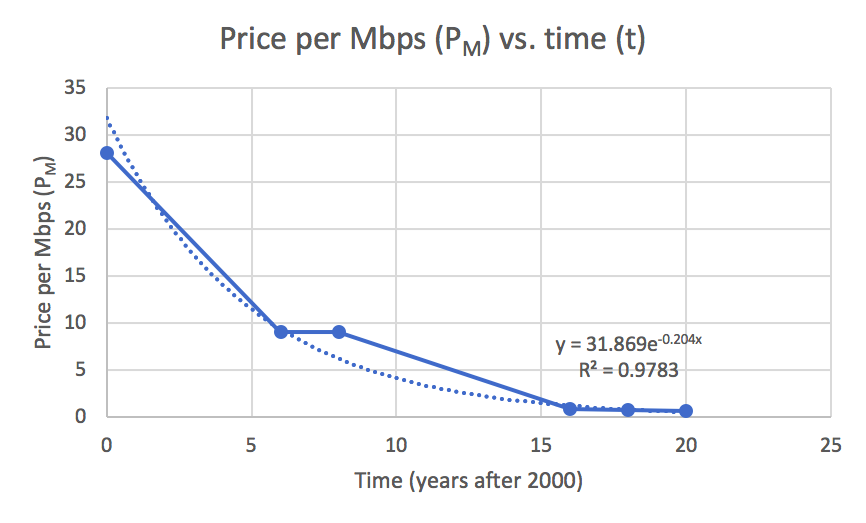
\includegraphics[width=9cm]{modelinga_image1}
    \caption{The model that can be used to predict the cost per unit of bandwidth in dollars per Mbps over the next 10 years. The value of R-squared was 0.9783, demonstrating the effectiveness of the model.}
    \label{fig:1}
    \end{minipage}
    
    \end{figure}
    
    A second data set was also found, with 18 data points, in another study [2] to create a second model, as shown below.
    
    \begin{center}
        
\begin{tabular}{|l|l|l|}
\hline
\multicolumn{3}{|c|}{Price per Mbps ($P_M$) vs time ($t$) — Table 2} \\ \hline
Time (years after 1998)   & Price per Mbps ($P_M$)   & \% decline  \\ \hline
0                         & 1200                  &             \\ \hline
1                         & 800                   & 33          \\ \hline
2                         & 675                   & 16          \\ \hline
3                         & 400                   & 41          \\ \hline
4                         & 200                   & 50          \\ \hline
5                         & 120                   & 40          \\ \hline
6                         & 90                    & 25          \\ \hline
7                         & 75                    & 17          \\ \hline
8                         & 50                    & 33          \\ \hline
9                         & 25                    & 50          \\ \hline
10                        & 12                    & 52          \\ \hline
11                        & 9                     & 25          \\ \hline
12                        & 5                     & 44          \\ \hline
13                        & 3.25                  & 35          \\ \hline
14                        & 2.34                  & 28          \\ \hline
15                        & 1.57                  & 33          \\ \hline
16                        & 0.94                  & 40          \\ \hline
17                        & 0.63                  & 33          \\ \hline
\end{tabular}

    \end{center}
	
	
	\begin{figure}[htp]
    \centering
    \begin{minipage}{9cm}
    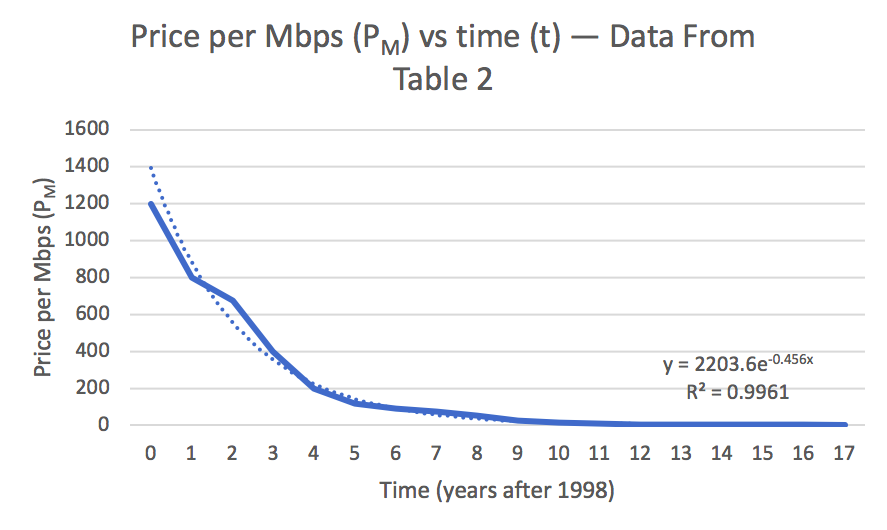
\includegraphics[width=9cm]{modelinga_image2}
    \caption{A second model that shows Price per Mbps vs time.}
    \label{fig:2}
    \end{minipage}
    \end{figure}
	
	While the R-squared value of this model was 0.9961—higher than the R-squared value of the first model—this second model cannot be used to extrapolate over the next 10 years. Still, it was useful in providing supporting evidence that the Price per Mbps decreases exponentially over time.

    Further, D2 provided values of Median Peak Download Speed (Mbps) and Median Monthly Price (\$) for various cities. For five cities, there were values for both 2012 and 2020. For these cities, the Median Monthly Price was divided by the Median Peak Download Speed (Mbps) to calculate the Price per Mbps ($P_M$). The percent change was similar to the percent change calculated in the previous two data sets, furthering the confidence in the model.
	
	
	\begin{center}
\begin{tabular}{|l|l|l|}
\hline
\multicolumn{3}{|c|}{Price per Mbps (PM) in 2012 and 2020} \\ \hline
2012            & 2020            & Percent Change (\%)    \\ \hline
2.082333333     & 0.23196         & 88.86057308            \\ \hline
1.787575758     & 0.188166667     & 89.4736396             \\ \hline
3.120909091     & 0.655172414     & 79.00700101            \\ \hline
2.949           & 0.27495         & 90.67650051            \\ \hline
2.098333333     & 0.4995          & 76.19539317            \\ \hline
\end{tabular}
\end{center}
	
    \subsubsection{Part II: United Kingdom}
    
    Price data on monthly internet plans for the United Kingdom were provided by data sets in D3. These monthly prices provided in a year were averaged to calculate a singular monthly value that could be used for all months in that given year. This method was used to find the prices for months in years from 2014 to 2019.

    The download speed data was gathered by Akamai from 2010 and 2017. Data gathered by Ookla was not available before 2017, and the source differed from Akamai in its measurement methodology, so it was omitted to maintain data continuity.

    To find the prices from years 2010 through 2013, a linear model was created from the price data based on year.

	\begin{figure}[htp]
    \centering
    \begin{minipage}{9cm}
    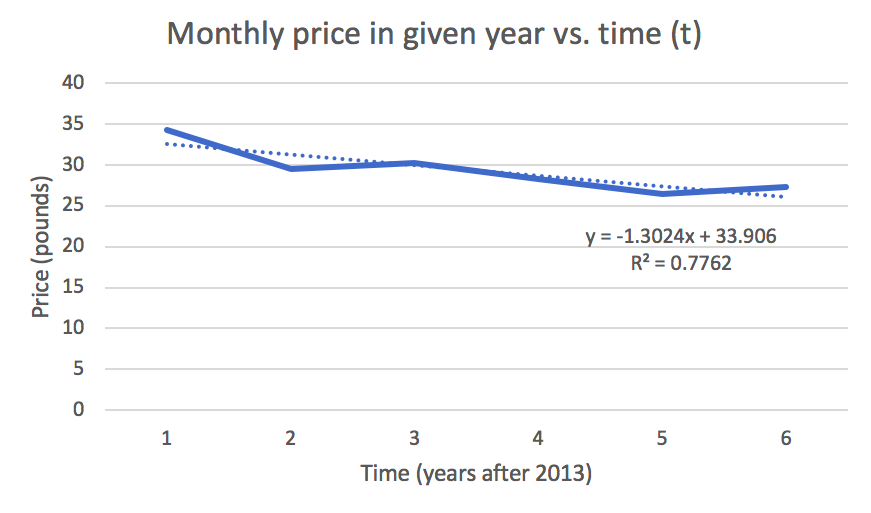
\includegraphics[width=9cm]{modelinga_image3}
    \caption{Monthly internet price (pounds) in UK in the years after 2013.}
    \label{fig:3}
    \end{minipage}
    \end{figure}
    
    This model was used to extrapolate prices from 2010 to 2013. Then, prices from 2010 through 2017 could be divided by the download speed to calculate $P_M$ and create the United Kingdom model.

% Please add the following required packages to your document preamble:
% \usepackage[table,xcdraw]{xcolor}
% If you use beamer only pass "xcolor=table" option, i.e. \documentclass[xcolor=table]{beamer}
\begin{center}
\begin{tabular}{|l|l|}
\hline
\multicolumn{1}{|c|}{Price}   & \multicolumn{1}{c|}{Speed (Mbps)} \\ \hline
{\color[HTML]{4472C4} 37.813} & 3.8                               \\ \hline
{\color[HTML]{4472C4} 36.511} & 4.6                               \\ \hline
{\color[HTML]{4472C4} 35.208} & 5.6                               \\ \hline
{\color[HTML]{4472C4} 33.906} & 7.9                               \\ \hline
34.25                         & 9.9                               \\ \hline
29.5                          & 11.6                              \\ \hline
30.25                         & 14.9                              \\ \hline
28.25                         & 16.9                              \\ \hline
\end{tabular}
\end{center}

\newcommand{\blue}{\color{blue}}
\newcommand{\black}{\color{black}}
The above data table shows the values used for the final UK model. The numbers in \blue blue \black were extrapolated.


    \begin{figure}[htp]
    \centering
    \begin{minipage}{9cm}
    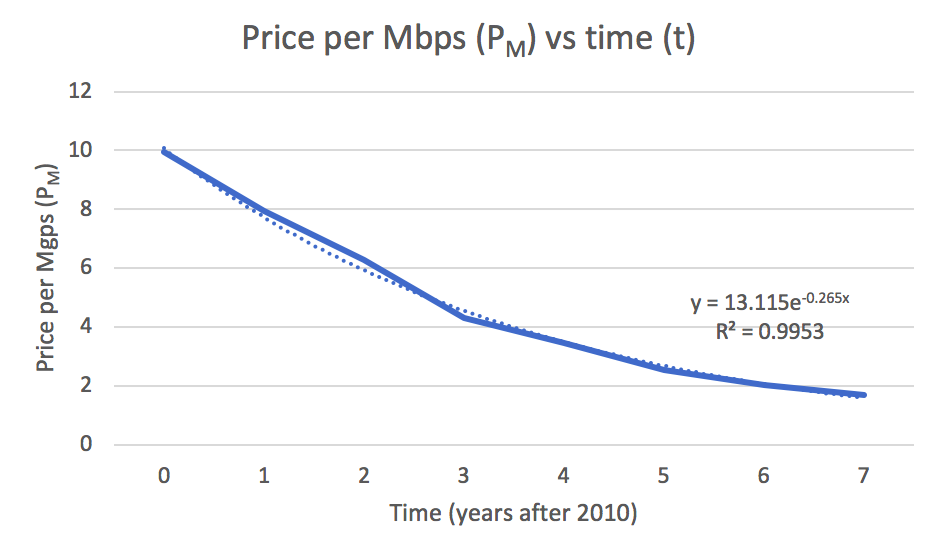
\includegraphics[width=9cm]{modelinga_image4}
    \caption{The final UK model that can be used to to predict the cost per unit of bandwidth in pounds per Mbps over the next 10 years in the UK.}
    \label{fig:4}
    \end{minipage}
    
    \end{figure}
   
   \pagebreak
   \subsection{Executing the Model}
   \subsubsection{Part I: United States}
   The model that was built for the United States utilized the equation $y = 31.869e^{-0.204x}$. The independent variable is the number of years after 2000, and the dependent variable is $P_M$. By plugging in values from 20 to 30, the cost per unit of bandwidth per Mbps can be found in any of the next 10 years.
   
   \begin{center}
\begin{tabular}{|c|c|}
\hline
\multicolumn{2}{|c|}{US Model — Value of PM over next 10 years} \\ \hline
x                          & y                                  \\ \hline
20                         & 0.538824023                        \\ \hline
21                         & 0.439390715                        \\ \hline
22                         & 0.358306595                        \\ \hline
23                         & 0.292185545                        \\ \hline
24                         & 0.238266318                        \\ \hline
25                         & 0.194297216                        \\ \hline
26                         & 0.158442069                        \\ \hline
27                         & 0.129203545                        \\ \hline
28                         & 0.105360629                        \\ \hline
29                         & 0.085917629                        \\ \hline
30                         & 0.070062593                        \\ \hline
\end{tabular}
\end{center}
    
    \subsubsection{Part II: United Kingdom}
    The model built for the UK utilized the equation $y = 13.115e^{-0.265x}$. The independent variable is the number of years after 2010, and the dependent variable is $P_M$. By plugging in values from 10 to 20, the cost per unit of bandwidth per Mbps (monthly) can be found in any of the next 10 years.
    
    \begin{center}
\begin{tabular}{|c|c|}
\hline
\multicolumn{2}{|c|}{UK Model — Value of PM over the next 10 years} \\ \hline
x                            & y                                    \\ \hline
10                           & 0.92659066                           \\ \hline
11                           & 0.71088587                           \\ \hline
12                           & 0.54539587                           \\ \hline
13                           & 0.41843095                           \\ \hline
14                           & 0.32102272                           \\ \hline
15                           & 0.24629054                           \\ \hline
16                           & 0.18895557                           \\ \hline
17                           & 0.14496784                           \\ \hline
18                           & 0.11122019                           \\ \hline
19                           & 0.08532879                           \\ \hline
20                           & 0.06546475                           \\ \hline
\end{tabular}
    \end{center}
    
    

    \subsection{Results and Discussion}
    \subsubsection{Strengths and Weaknesses}

    The exponential regression model provides a superior estimate based on past data used to extrapolate into the future. Its simplicity reduces the background effects of minor variables while still allowing them to affect data through past values. The R-squared values of the models are extremely high, suggesting a level of confidence in the model. However, future predictions are seldom accurate and perfect accuracy is impossible to achieve with predictive models.

    The data for the first model comes from 6 data points taken over a course of 20 years, from 2000 to 2020, while the timeframe of the extrapolation has a duration of 10 years. While the time frame seems sufficient, an ideal model would have more data points 

    The data for the second model comes from 8 data points taken over the course of 7 years. In an ideal model, the time frame may need to be lengthened to improve accuracy and decrease variability in the data. There are further limitations to this model because the invention of the internet is relatively recent, and data on internet traffic in its early days is limited.

    \subsubsection{Sensitivity Analysis}
    Since both of the models model were found by dividing price by download speed, these two parameters can be found in this equation:
    
    $$P_M(t)=\frac{P(t)}{s(t)}$$
    
    It was found that $P_M(t)$ experiences exponential decay as time increases. The data for $P_D(t)$ showed that the price decreased slightly over time. For $P_P(t)$, the model showed that the price was decreasing linearly. $S(t)$, the download speed, generally varies with internet speeds. Since internet speeds have increased dramatically and exponentially over the last 20 years, the finding that $P_M(t)$ decreases exponentially makes mathematical sense. If a parameter—$P(t)$, for example—was to change slightly, it would not have a significant effect on the model. However, if the behavior of $P(t)$ or $s(t)$ in a fundamental way, the model would no longer be accurate.


\pagebreak
\begin{thebibliography}{2}

\bibitem{} 
https://www.ncta.com/industry-data

\bibitem{}
https://drpeering.net/white-papers/Internet-Transit-Pricing-Historical-And-Projected.php


\end{thebibliography}
